\documentclass{article}
\usepackage{tikz}

\begin{document}
\section{A TikZ example}

\begin{figure}
  \centering
  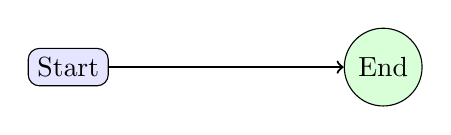
\begin{tikzpicture}
    \node[draw, rounded corners, fill=blue!10] (start) at (0,0) {Start};
    \node[draw, circle, fill=green!15] (finish) at (4,0) {End};
    \draw[->, thick] (start) -- (finish);
  \end{tikzpicture}
  \caption{Two nodes connected by an arrow.}
\end{figure}
\end{document}
